\documentclass[12pt]{article}

\usepackage[margin=2.5cm]{geometry}
\usepackage{graphicx}
\usepackage{natbib}
%correct punctuation for MBE
\bibpunct[,]{(}{)}{;}{a}{}{,}

\usepackage{amsmath}

\renewcommand{\bottomfraction}{.9}
\renewcommand{\topfraction}{.9}
\renewcommand{\textfraction}{0.1}
\renewcommand{\floatpagefraction}{.9}

\linespread{1.5}
\begin{document}

\title{\textbf{Predicting virus-receptor mutant binding by molecular dynamics simulation}}
\author{Austin G. Meyer$^{1,2,4*}$, Sara L. Sawyer$^{3}$, Andrew D. Ellington$^{2}$,\\and Claus O. Wilke$^{1}$}
\date{}

\maketitle
\noindent
Address:\\
$^1$Section of Integrative Biology, Institute for Cellular and Molecular
Biology, and Center for Computational Biology and Bioinformatics. The University
of Texas at Austin, Austin, TX 78712, USA.\\
$^2$Department of Chemistry and Biochemistry, Institute for Cellular and Molecular 
Biology, The University of Texas at Austin, Austin, TX 78712, USA.\\
$^3$Section of Molecular Genetics and Microbiology, Institute for Cellular and Molecular 
Biology, The University of Texas at Austin, Austin, TX 78712, USA.\\
$^4$School of Medicine, Texas Tech University Health Sciences Center, 
Lubbock, TX 79430, USA.\\

\bigskip
\noindent
$^*$Corresponding author\\
$\phantom{^*}$Email: austin.meyer@utexas.edu\\
$\phantom{^*}$Phone: +1 512 971 0123\\

\bigskip
\noindent
Manuscript type: research article

\bigskip
\noindent Keywords: protein--protein interaction, molecular dynamics, arenavirus, machupo

\newpage

\begin{abstract}

Existing computational methods to predict protein--protein interaction affinity often perform poorly in important test cases. In particular, the effects of multiple mutations, non-alanine substitutions, and flexible loops are difficult to predict with available tools and protocols. We present here a new method to interrogate affinity differences resulting from mutations in a host-virus protein--protein interface. Our method is based on extensive non-equilibrium all-atom simulations: We computationally pull the machupo virus (MACV) spike glycoprotein (GP1) away from the human transferrin receptor (hTfR1) and estimate affinity using the maximum applied force during a pulling simulation and the area under the force-versus-distance curve. We find that these quantities provide novel biophysical insight into the GP1/hTfR1 interaction. First, with no prior knowledge of the system we can differentiate among wild-type and mutant complexes. Second, although the static co-crystal structure shows two large hydrogen-bonding networks in the GP1/hTfR1 interface, our simulations indicate that only one of them is critical for the binding interaction. Third, one viral site known to be critical for infection may mark an important evolutionary suppressor site for infection-resistant hTfR1 mutants. Finally, our method provides an elegant framework to compare the effects of multiple mutations, individually and jointly, on protein--protein interactions.
\end{abstract}

\section*{Introduction}

The computational prediction of mutational effects on protein--protein interactions remains a challenging problem. Several methods are available to perform an energy difference calculation from an experimentally determined co-crystal structure. For example, computational alanine-scanning can be performed rapidly, with relatively low computational cost \citep{Grant2011,Kortemme2004}. However, such methods calculate the relative contribution to overall energy for each amino acid in a protein. They do not probe the interface directly, but rather calculate the total energy with each substitution \citep{Grant2011,Kortemme2004}. Alternative approaches have been developed using machine learning, training coefficients in a weighted equation containing geometric and energetic parameters \citep{Vreven2011,Vreven2012,Bajaj2011,Hwang2010}. Unfortunately, such machine-learning approaches often suffer in novel applications, for which available training sets are small or non-existent. As such, these methods are poorly suited for most host-virus protein--protein systems. By contrast, first principles methods offer the chance to forgo training. However, the currently available methods such as free energy perturbation (FEP) and thermodynamic integration (TI) rely on a two state model that phases directly from one three dimensional protein model to another with no intermediate transition states \citep{Gilson1997,Lu2004}. Thus, they can quickly lose physiological relevance as the two proteins become more dissimilar and as a result are largely limited to testing only sequential point mutants. 

Here we propose a new method to probe mutational effects in protein--protein interactions directly, by pulling two proteins apart that are initially bound in a complex. We impart a pulling force within an all-atom molecular dynamics simulation on one member of the complex while the other is held in place. Then, we measure the force required for dissociation. As a proxy for relative binding affinity, we use the maximum applied force (MAF) required for separation and the area under the force-versus-distance curve (AUC). 

We applied our method to interrogate the interaction between machupo virus (MACV) spike glycoprotein (GP1) and the human transferrin receptor (hTfR1) \citep{Abraham2010,Charrel2003}. Machupo is a negative-sense RNA virus of the arenavirus family \citep{Charrel2003}. Worldwide arenaviruses represent a significant source of emerging zoonotic diseases for the human population \citep{Charrel2003}. Members of the arenavirus family include the lassa fever virus endemic to West Africa, the lymphochoriomeningitis virus (LCMV) endemic to rodents in several areas of the United States, and the guanarito, junin and machupo viruses endemic to rodents in South America \citep{Charrel2003}. The South American arenaviruses typically infect humans after rodent contamination and cause a devastating hemorrhagic fever with very high mortality \citep{Charrel2003}.

The hTfR1 is the primary receptor used by MACV for binding its host cell prior to infection. The hTfR1 protein contains three extracellular domains with the two more basilar domains serving most of the endogenous, transferrin-binding function \citep{Abraham2010,Rad20112}. Cellular entry is initiated by GP1 binding to the apical domain of hTfR1. Previous work has indicated that the GP1/hTfR1 binding interaction is the primary determinant of viral infectivity \citep{Rad20111,Rad20112}. The co-crystal structure shows that a 15 amino acid flexible loop on GP1 is responsible for viral binding \citep{Abraham2010,Rad20112}, and many of the interface interactions are mediated by extensive hydrogen-bonding networks \citep{Abraham2010}. Furthermore, the high affinity interaction between GP1 and hTfR1 forces the normally flexible loop in the apical domain of hTfR1 into a rigid beta-pleated sheet domain. Experimental alanine-scanning and whole cell infectivity assays have identified several sites in both GP1 and hTfR1 that are probably critical for establishing infection \citep{Rad20111,Rad20112}.

We applied our method to wild type (WT) and mutant complexes, and found that we could resolve relative differences in unbinding and predict significant affinity changes. At sites known to be important for successful viral entry, we found that the biochemical cause of reduced infectivity is often not as simple as the static structure suggests. For example, the static structure shows a hydrogen-bonding network connected to site Asn348 in hTfR1. According to our simulations, this network likely does not affect binding affinity. Our study offers an all-atom steered molecular dynamic approach to avoid the pitfalls of several existing methods used to evaluate mutations in host-virus protein--protein interfaces.

\section*{Materials and Methods}

\subsection*{System Modeling}

We used the protein visualization software PyMOL \citep{PyMOL} to remove residues 121-190, 301-329, and 383-756 in the hTfR1. No residues were removed from the viral protein. We also removed 10 sugar residues from the native structure.

After system reduction, the Visual Molecular Dynamics (VMD) \citep{Humphrey1996} package along with its system of back-ends was used for all subsequent modeling. The Orient add-on package allowed us to rotate the system axis such that the direction of steering was oriented directly down the z-axis. De-glycosylation simplified the system such that Autopsf could easily find the chain terminations and patch them appropriately. The Solvate package was used to generate a TIP3P water model with a 5 \AA ngstrom buffer (relative to the maximum dimensions of the proteins) on all sides except down the positive z-axis where a 20 \AA ngstrom buffer was created. Finally, we used the Autoionize package to place 150 millimolar NaCl and neutralize the total system charge. In the end, each modeled system had approximately 28,000 atoms.

\subsection*{Equilibration}

NAMD was used for all simulations in this study \citep{Phillips2005}. In addition to the modeled system, for equilibration we generated a configuration file that fixed the $\alpha$-carbon backbone. This was accomplished by setting $\beta = 1$. Further, we generated a configuration file with fixed $\alpha$-carbon atoms at residues 41-92 (numbered linearly, in this case, starting at 1 for the first amino acid as was required for VMD) in the hTfR1. The second file was used to affix a harmonic restraint, thus preventing any unfolding due to system reduction. More importantly, the harmonic restraint allowed the protein complex to equilibrate while preventing any drift from its predefined orientation. Finally, we calculated the system center and dimensions for use in molecular dynamics settings.

We used the Charmm27 \citep{Brooks1983} all-atom force field. The initial system temperature was set to 310K. Several typical MD settings were used including switching and cutoff. In addition, we used a 2 femtosecond time step with rigid bonds (the exact configuration is provided in the supplement). We used periodic boundary conditions with the particle mesh ewald (PME) method of computing full system electrostatics outside of the explicit box. Furthermore, we used a group pressure cell, flexible box, and langevin piston during equilibration. Finally, a harmonic restraint (called harmonic constraint in VMD) was set as stated previously.

To start the simulation, the langevin piston was switched off and the system was minimized for 1000 steps. Next, the fixed backbone was released, and the system was minimized for an additional 1000 time steps. Subsequently, the system was released into all-atom molecular dynamics for 3000 steps. Finally, the langevin piston was turned on and the system was simulated for 2 ns (1,000,000 steps) of chemical time. For each mutant, twenty independent replicates were run with an identical protocol.

\subsection*{Steered Molecular Dynamics}

Following equilibration, the final state of each simulation was used to generate a configuration file fixing the $\alpha$-carbon on residues 1, 58, 73-83, 96, 136, 137, 138, and 161 (again with linear numbering) in the hTfR1. Also, the $\alpha$-carbon of all residues (163-318 in linear numbering) in the GP1 were given an occupancy of 1, indicating they had an applied force during the simulation. 

In every way possible the subsequent steering simulation had the same parameters as the equilibration simulation. Thus, the steered molecular dynamics (SMD) \citep{Is2001B} simulation was a typical restart with slightly different settings. Periodic boundary conditions were incorporated as part of the system and PME was again used to approximate full system electrostatics. In addition, we first tuned the pulling velocity for practical time considerations. Subsequently, the spring constant was adjusted to ensure sufficient signal to noise with the given velocity. As a result, the spring constant was set to 5 (units), velocity set to 2 (units), and direction down the positive $z$-axis.

Finally, SMD was run for 15 ns (7,500,000 time steps) of chemical time. For each simulation, we randomly selected one of the equilibration runs for restart. We ran 50 replicate simulations per mutant. All GP1/hTfR1 complexes separated by greater than 4 \AA ngstroms and many separated to 10 or more.

To leave the final trajectory of a tractable size, only 1000 evenly spaced frames were retained from each simulation, leaving a final trajectory size of 323 MB. See the supplemental movie for a representative unbinding trajectory. Initial development of the SMD protocol was carried out on the Lonestar cluster at the Texas Advanced Computing Center (TACC). All production SMD simulations were performed on the Hrothgar cluster at Texas Tech University, using NAMD 2.9. Each simulation was parallelized over 60 computational cores and utilized approximately 20 hours of computing time. The total chemical time simulated for this project was nearly 10 $\mu$s, requiring slightly over 1 million cpu-hours.

\subsection*{Post-processing}

The python packages MDAnalysis \citep{Agrawal2011} and ProDy \citep{Bakan2011} were both used at various points in post-processing. The molecular trajectory (comprising the atomic coordinates per time) was parsed to compute the center-of-mass for each of the two complexes. The starting center-of-mass distance was set to zero and the distance was re-computed at each time step relative to the starting distance. The force is output directly to the standard log file.

The statistical package R was used for all further analysis and visualization. Each of the 50 independent trajectories per mutant produced a fairly noisy force curve. To reduce the noise, we averaged each point with a 75 point interpolation window. The window ensured that the averaged MAF was never cut off near the beginning of the simulation due to lost time steps (caused by averaging). The two primary descriptive statistics we used were maximum interpolated applied force (MAF) and total area under the interpolated curve (AUC). We used the pairwise.t.test function with the FDR p-value correction to test for significance. The ggplot \citep{ggplot} package was used to generate most of the figures. 

\section*{Results}

\subsection*{The GP1/hTfR1 system}

The GP1/hTfR1 interface marks a particularly important and useful test system. There are several sites on both the human and viral protein known to affect the infectivity phenotype of MACV. Virtually all of the important sites have been mapped by \textit{in vitro} flow-cytometry based infectivity assays. The GP1/hTfR1 interface appears not to be dominated by one particular type of interaction (electrostatics, hydrogen-bonding, or van der Waals). In addition, much of the binding domain on hTfR1 is on a flexible loop and undergoes a large structural rearrangement upon binding, making many other computational techniques \citep{Grant2011,Kortemme2004} only marginally useful. The complex nature of this interface represents a particularly difficult challenge for traditional computational analysis. 

For our experiments, we used the experimentally determined GP1/hTfR1 structure (PDBID: 3KAS) \citep{Abraham2010}. The apical domain of hTfR1 interacts directly with GP1 while the other two domains are closer to the cell membrane and have essentially no interaction with GP1. The biophysical independence of the apical domain allowed us to isolate it without significantly affecting the GP1/hTfR1 interaction. Figure~\ref{fig:protein_comparison} shows a model of the initial structure and that of the pared structure. Although GP1 has several glycosylatable residues, we opted to use the de-glycosylated protein for this study. The complexity of correctly parameterizing diverse sugar moieties is outside of the scope of this paper. Furthermore, although it is known that GP1 is glycosylated, and some of those sugars contact hTfR1, the effect of those contacts \textit{in vivo} is still unresolved \citep{Abraham2010}.

\subsection*{Steered molecular dynamics simulations}
To ensure a natural solution structure, we performed an initial equilibration phase to reduce the intrinsic crystallization distortions. First, we generated a physically realistic simulation world around the protein complex. The environment included an explicitly modeled bath of water, and a physiologically relevant concentration of ions. Next, with a fixed $\alpha$-carbon backbone we carried out successive rounds of energy minimization, followed by heating, and backbone release. Last,  with minimal restraints a short round of all-atom molecular dynamics \citep{Cuendet2008} was performed. We used the final state from each equilibrated system to restart another MD simulation. For SMD, at the centroid of several atoms a force was applied to a single point in GP1. By using a known spring constant, and pulling with a constant velocity, we could calculate the applied force during protein--protein dissociation \citep{Cuendet2008,Cuendet2011}. A typical averaged force curve comparison can be seen in Figure~\ref{fig:force_curve}. The force curves for each mutant were smoothed either by averaging over many replicates as in Figure~\ref{fig:force_curve} or by selecting an interpolation window for averaging. The latter approach was used for statistical analysis. In addition, to minimize the computational time in unproductive molecular dynamics, we shortened the simulation time such that the interaction just barely dropped to zero near the end of each run. As seen in Figure~\ref{fig:force_curve}, this distance was relatively consistent among mutants. The supplementary movie visually illustrates the separation distance between peptide domains. The quantities MAF and AUC were derived from the force versus distances curves. Their summary statistics are reported in Table~\ref{tab:summary_statistics}. As we are more interested in the phenotypic impact of interface mutations we avoided many of the more physically rigorous, but technically complicated calculations that are possible with SMD \citep{Is2001A,Is2001B}.

Before systematically applying SMD to the GP1/hTfR1 interaction, we needed to ensure the method was sufficiently sensitive to distinguish between relatively minor point mutations. While SMD has been applied previously to measure the binding energy of high-affinity T-cell receptor interactions \citep{Cuendet2008,Cuendet2011}, to our knowledge the method has never been used previously to parse small differences in a complex energy landscape. For this initial sensitivity analysis, we tested alanine substitutions congruent with the traditional experimental and computational approach. Several residues on both proteins appear to mediate putative hydrogen-bonding interactions. We selected three sites for alanine substitutions: Tyr211 and Asn348 in the hTfR1 and vArg111 in MACV. For notation purposes, the viral site is always referred to with a preceding `v'. According to the static complex \citep{Abraham2010}, Tyr211 and vArg111 are involved in one hydrogen-bonding network and Asn348 is involved in a second, distinct hydrogen-bonding network.

We found that relative to WT, one alanine mutation (Tyr211Ala) produced a very large and statistically significant difference in the MAF and AUC (Figure~\ref{fig:force_curve}, Table~\ref{tab:pairwise_differences}), while the other two did not (Table~\ref{tab:pairwise_differences}). From these results, we concluded that our method can indeed successfully distinguish individual mutants from WT, and that alanine substitutions at Asn348 and vArg111 may have little effect on binding affinity (see below for further discussion). When considering additional mutants (also discussed below), we found that MAF was generally sufficient to distinguish mutants (Tables~\ref{tab:pairwise_differences} and~\ref{tab:MAF_p}), and AUC was able to add a few more statistically significant differences (Table~\ref{tab:AUC_p}). In general, however, MAF seemed to be the more sensitive statistic than AUC.

\subsection*{Comparative analysis of the GP1/hTfR1 interface}

Considering the involvement of extended hydrogen-bonding networks in the GP1/hTfR1 interface, it was not clear that individual alanine mutations, even those that should destroy such networks, would significantly change the strength of interaction. One major advantage of first principles simulations is the ability to test mutations other than alanine without additional underlying assumptions in the energy function. We made additional mutations based on biochemical intuition or available experimental data to chemically diverse amino acids including tryptophan, lysine, aspartate, and threonine. Several mutations caused significant relative affinity changes. In addition, to detect synergistic effects, we tested several double mutants where both mutations appeared to cause reduced binding. Then, we compared the size of those differences to reduced binding single mutants (Figure~\ref{fig:sensitivity}).

In total, we tested 7 point mutants and 3 double mutants in addition to the WT complex (Table~\ref{tab:summary_statistics}). The largest single-mutant impact was seen for a mutation to alanine at site Tyr211 in the hTfR1 ($ p < 0.001 $).  Several mutations at this site have proven capable of causing loss-of-infection, according to \textit{in vitro} flow-cytometry infection assays or known host-range limitations \citep{Rad2008,Rad20111,Rad20112}. Most likely, this effect is caused by the destruction of a critical hydrogen bond to Ser113 in GP1. The lost hydrogen bond would lead to the subsequent loss of a large hydrogen-bonding network seen in the crystal structure \citep{Abraham2010}. In agreement with the static structure, our molecular dynamics simulations show Tyr211 is involved in a large hydrogen-bonding network (results not shown). 

Although Tyr211Ala appears to have a large impact on binding affinity, the single mutant provided little underlying biochemical rationale. Since alanine is both smaller than tyrosine and also incapable of participating in hydrogen-bond interactions, we tested further mutations to identify the critical biochemical difference responsible for loss of binding affinity. In particular, we substituted smaller side chains that, like tyrosine, were capable of hydrogen bonding. We chose Tyr211Asp and Tyr211Thr, two mutations that have been discussed in the context of selection pressure on hosts in rodent populations \citep{Rad2008,Rad20111,Rad20112}. Both mutations proved incapable of causing reduced binding affinity in our simulations. In fact, they caused a significant increase in relative binding affinity (Figure~\ref{fig:sensitivity} and Table~\ref{tab:MAF_p}). This outcome is not surprising, if we consider that Tyr211 participates in a bonded network rather than independently. Combined with some biochemical intuition, these results suggest that mutations to other polar residues would likely not affect the dynamics of binding directly.

We also simulated several point mutations at Asn348 in the hTfR1. Asn348Lys is reported in the literature to cause reduced infectivity \textit{in vivo} \citep{Rad2008,Abraham2010}. Further, in the crystal structure two residues on GP1 and at least three on hTfR1 are involved in a fairly extensive hydrogen-bonding network. As discussed above, the alanine mutation at this site showed no significant difference in MAF or AUC from WT (Tables~\ref{tab:MAF_p} and ~\ref{tab:AUC_p}). In addition, the Asn348Lys mutation showed no significant difference from WT, and neither did Asn348Trp. (For both of these mutations, mean MAF and mean AUC was lower than for WT, however. See Table~\ref{tab:summary_statistics})  On the other hand, there was a detectable difference between Asn348Ala and Asn348Lys (Tables~\ref{tab:MAF_p} and~\ref{tab:AUC_p}), with Asn348Lys being a weaker binder. Moreover, Asn348Trp showed nearly identical results to Asn348Lys. These results suggest that, in contrast to Tyr211, the critical difference at position 348 in hTfR1 is size exclusion rather than the destruction of a hydrogen-bonding network. The mutations to large amino acids (Asn348Trp and Asn348Lys) produced nearly identical affinity changes, whereas the mutations to amino acids not capable of hydrogen bonding (Asn348Ala and Asn348Trp) produced significantly different affinity changes (Table~\ref{tab:pairwise_differences}). To check the consistency of our results, we hypothesized that the combination of Tyr211Ala and Asn348Trp, being chemically disconnected in two different hydrogen-bonding networks, would lead to a synergistic loss-of-binding. As expected, the double mutant was the weakest binding mutant tested ($ p < 10^{-6} $) (Tables~\ref{tab:MAF_p} and~\ref{tab:AUC_p}) in this study. Further, according to MAF (but not AUC), the combination of Tyr211Ala and Asn348Trp also showed significantly weaker binding than Tyr211Ala by itself (Tables~\ref{tab:MAF_p} and~\ref{tab:AUC_p}). We suspect that the effect of Asn348Trp alone is near the limit of detection using our method. A larger number of replicates would possibly have resolved affinity differences between Asn348Trp and WT or other mutants more consistently.

Last, we further analyzed a single mutation in GP1, vArg111Ala. It has been reported that vArg111Ala causes a loss-of-infection during \textit{in vitro} infectivity assays \citep{Rad20112}. As mentioned in the previous subsection, in our simulations this mutant showed no significant change in either MAF or AUC (Tables~\ref{tab:MAF_p} and~\ref{tab:AUC_p}), even though both quantities were, on average, lower than in WT (Table~\ref{tab:summary_statistics}). This result was somewhat surprising, since Tyr211Ala, presumably disrupting the same hydrogen-bonding network as vArg111Ala, displayed a significant reduction in affinity. To probe the interaction between position 111 in the GP1 and position 211 in the hTfR1 further, we also tested the double mutant vArg111Ala/Tyr211Ala. This double mutant showed affinity indistinguishable from WT and significantly higher than Tyr211Ala alone  (Table~\ref{tab:pairwise_differences}). Thus, vArg111Ala in the GP1 appeared capable of suppressing the loss-of-binding caused by Tyr211Ala. This result shows that the two sites do indeed interact significantly, and that replacing the hydrogen-bonding network at these sites with a hydrophobic interaction leads to comparable binding affinity.

\section*{Discussion}
We have applied a method utilizing steering forces in all-atom molecular dynamics simulations to evaluate the effects of mutations at the GP1/hTfR1 interface. We modeled mutations at several sites in the GP1/hTfR1 interface, and verified that our computational protocol was sensitive enough to distinguish point mutants in hTfR1. Further, we identified two test statistics, MAF and AUC, that can be used as proxies for binding affinity. We systematically tested several point mutations to understand their contribution to the binding interaction. In the case of Asn348Lys, we have shown that the static structure provides little insight into why this mutation causes loss-of-infectivity \textit{in vivo}. While Asn348 appears to be involved in a hydrogen-bonding network in the static structure, loss of binding affinity at that site is actually caused by size and charge restriction. Further, we have shown that the cause of diminished infectivity in the viral single-mutant vArg111Ala may not be due to binding-energy differences. We also found that a negatively polar residue at site 211 in hTfR1 is absolutely critical for a tight binding interaction. Any non-polar mutation at Tyr211 in hTfR1 is likely to completely halt viral entry and dramatically decrease the chances of MACV infection. However, our data suggest that the viral mutation vArg111Ala may restore the infective potential of MACV that was previously destroyed by a Tyr211Ala hTfR1 mutation.

By extending the SMD technique to investigate a protein--protein interaction we have, in many ways, changed the scope of its application. Traditionally this technique is either applied to compute equilibrium quantities via a non-equilibrium approximation \citep{Park2003,Park2004,Buch2011,Giorgino2012}, used to estimate protein stability through unfolding \citep{Lu1999}, or used to calculate the absolute free energy of small molecule ligand binding \citep{Dixit2001}. Likewise, others have used SMD to understand the process of binding and unbinding at a resolution unmatched by experiment \citep{Cuendet2011,Giorgino2012}. And still others aimed at more esoteric problems apply driving forces to untie polypeptide knots in toy systems \citep{Sulkowska2010}. Here, we have shown that SMD can provide some insight into the \textit{relative} strength of protein--protein interactions. In contrast to more traditional absolute affinity calculations, relative binding is much more useful for experimental application. Further, our method complements whole cell infectivity assays, which demonstrate phenotypic effects but do not provide biochemical mechanisms. Via SMD, one can separate mutations whose likely effect is altered binding affinity from mutations that may affect other factors such as protein expression, protein folding, or interactions with other proteins not considered in the simulation. Thus, SMD may open avenues for subsequent experimental work.

Our findings rationalize several effects observed in both infectivity data and rodent populations \citep{Rad2008,Rad20111}. We found that some substitutions at positions 211 and 348 did negatively affect the strength of viral binding. In the two cases, the computational data suggests that the reason and nature of the effects are very different. Congruent with infectivity data, mutations at Tyr211 often have a dramatic effect on receptor binding \citep{Rad2008,Rad20111}. Tyr211Ala alone produces such a large decrease in affinity that it can be easily distinguished from the WT complex. Structural analysis reveals that the biochemical cause involves the destruction of a critical hydrogen-bonding network with Ser113 and vArg111 in GP1. Further, Tyr211Asp and Tyr211Thr were easily resolved from the WT complex, but they appear to cause an increase in affinity. As a result, we predict experimental structural analysis will show Tyr211Asp and Tyr211Thr mutations cause a relatively dramatic tertiary structure deviation. Given that our model starts from an associated complex, it is not surprising that Tyr211Asp would cause increased rather than decreased affinity. Aspartate is charged rather than polar at physiological pH and its shorter side chain means the proteins would be pulled in closer apposition. Nevertheless, our results show Tyr211, or some other amino acid that is capable of hydrogen bonding, is necessary for a stable hydrogen-bonding network leading to efficient binding. Moreover, the cause of decreased infectivity seen in rodent populations with the Tyr211Asp mutation is not a simple change in binding affinity.

Previous work has shown that the hTfR1 mutation Asn348Lys is capable of producing decreased infectivity \emph{in vitro} \citep{Rad2008,Rad20111}. Moreover, the molecular model based on x-ray diffraction data suggests destruction of a second hydrogen-bonding network as the cause \citep{Abraham2010}. In our simulations no individual point mutation at Asn348 showed a significantly different affinity from the WT complex. Moreover, the mutation Asn348Ala resulted in an average MAF that was virtually identical to WT hTfR1 (Table~\ref{tab:pairwise_differences}). Thus, the putative hydrogen-bonding network involving Asn348 is probably a crystallization artifact. Even when paired with the highly destructive Tyr211Ala mutation, Asn348Ala was refractory to changes in binding affinity. By contrast, when Tyr211Ala was paired with large (Trp) and positively charged (Lys) substitutions at position 348, the result was a larger than expected synergistic difference. That is, the double mutant Tyr211Ala/Asn348Trp caused a much larger decrease in binding than we expected from either mutation individually. Moreover, although Asn348Trp and Asn348Lys individually failed to be distinguishable from WT hTfR1, they both caused a mean reduction in MAF and produced larger than expected synergistic effects. This data suggests that site 348 is size and charge restricted. Any mutation to a very large or positively charged side chain will likely produce decreased infectivity.

The GP1 mutation vArg111Ala causes a loss-of-infection during \textit{in vitro} infectivity assays \citep{Rad20112}, yet it was indistinguishable from the WT complex in our simulations. We suspected that this result was primarily caused by a lack of sensitivity of our method, since vArg111's binding orientation near Tyr211 and involvement in the critical hydrogen-bonding network strongly suggested that mutations at that site should have an effect on binding affinity. As an alternative way to test this hypothesis, we evaluated whether we could introduce a suppressor mutant at site vArg111. We introduced vArg111Ala jointly with Tyr211Ala, thus effectively replacing a hydrogen-bonding network with a hydrophobic interaction. Although Tyr211Ala was the most disruptive single mutant we tested, vArg111Ala in the GP1 was able to restore mean MAF to WT levels (Table~\ref{tab:summary_statistics}), and to levels significantly higher than observed for Tyr211Ala alone. As mutations at hTfR1 site 211 are known to reduce infectivity \emph{in vitro} and \emph{in vivo}, it is possible that vArg111 in GP1 can serve as a supressor site for compensatory MACV mutations. Thus, this site may be critically important for surveillance in the rodent population.

Although our computational predictions largely agreed with the available literature, some mutations that are reported to cause reduced infectivity in experimental systems (most notably vArg111Ala and Asn348Lys, discussed above) were indistinguishable from the WT complex in our simulations. We would like to emphasize here that we cannot expect perfect agreement. While we have shown that our method can distinguish individual point mutations, we do not know the limit of detection with our method. It is possible that some mutants display measurable phenotypic effects in experiments yet appear identical under our method. More extensive sampling or refinement of the simulation protocol could help to differentiate such mutants (see also next paragraph). In addition, the available experimental data for the GP1/hTfR1 system were generally obtained from infection assays, not binding assays. There are several reasons other than binding due to which a viral mutation may cause a phenotypic difference in infectivity. First, from infectivity experiments it is not clear the extent to which a protein is grossly or partially misfolded. An additional analytical step with circular dichroism or an analogous technique may further clarify large-scale folding differences. Second, since we start with a bound structure, any changes that may dramatically affect the rate of association (different folds, trafficking issues, etc.) would be underestimated by our method. Third, although it is tempting to think diminished infectivity should correlate strongly with decreased binding affinity, it is likely that dramatically increased binding affinity would prohibit cellular membrane detachment after viral invasion. As a result, the virus would be prevented from reaching its replication compartment (which is the cytosol in the case of Machupo) and could not reproduce.

As with any structural approach, we are constrained to start our computational model system from a static structure. One unfortunate reality in structural biology is poor resolution/discrimination at particularly long and flexible amino acid side chains. In addition, the number of acceptable side-chain rotamers increases in large amino acids. As a consequence there could be many untested starting conformations. Although we believe we have minimized unsampled conformations here, such an issue could be overcome with a sufficiently large number of SMD starting models. Of course, increasing sampling in this case comes at significant computational cost. There are a few additional challenges for investigating host-virus interaction via molecular dynamics simulation. As with any atomistic simulation, there is going to be a fairly large noise to signal ratio. To reduce noise, one could further customize each simulation, e.g. by determining the optimal pulling speed. Furthermore, larger amounts of computational resources will have a direct and powerful impact on the strength of any atomistic study \citep{Shaw2012}. Such resources could come in the form of increased compute time, improved code, or customized hardware for floating point operations \citep{Shaw2011}. With improved resources, we could investigate thousands of individual permutations in the GP1/hTfR1 binding interface. Going forward, we believe that all-atom molecular dynamics simulations can become an increasingly viable approach for protein interaction studies. 

Making accurate predictions regarding the effects of non-alanine mutations at protein--protein interfaces remains  challenging. The main obstacle is the enormous number of chemically allowed three dimensional configurations in proteins \citep{Gumbart2012}. In theory, one could carry out all-atom simulations from physical first principles \citep{Gumbart2012} for very long time periods. After equilibrium is reached in such simulations, one could then compute a binding constant by observing the fractional association/dissociation time among two proteins. Unfortunately, due to limited computational power and available methods, reaching equilibrium with a simulated protein system is truly a herculean task and is essentially impossible at this time \citep{Gumbart2012}. There are two broadly useful computational approaches that avoid first-principles equilibrium simulations. First, to reduce computational complexity several studies have used rigid body docking and machine learning \citep{Vreven2011,Vreven2012,Bajaj2011,Hwang2010}. While these approaches can work well in certain scenarios, they often underperform in applications to novel systems, due to their dependence on available training data. Second, hybrid approaches exist that exploit non-equilibrium calculations within the context of all atom simulations \citep{Dixit2001,Is2001A,Is2001B,Park2004,Grant2011,Kortemme2004,Gumbart2012}. However, to date most of these methods have not been applied to protein--protein interactions (but rather to simpler scenarios such as protein--ligand interactions). What we have shown here is that hybrid non-equilibrium approaches can provide a useful and practical tool in studying protein--protein interactions.

We have probed the biochemical effects of mutations at the host-virus interface between MACV and its human receptor. We applied an approach that imparts forces in an all-atom molecular dynamics (MD) simulation to drive the system through equilibrium. Our work has shown that with relatively modest computing resources it is possible to use MD simulations to investigate point mutations in the GP1/hTfR1 interface. In most cases, a double mutant was easily sufficient to resolve a difference in relative affinity. Moreover, relative to the WT complex one point mutant was capable of producing a large decrease in binding affinity. We applied our technique to the WT complex and 10 mutations in the GP1/hTfR1 interface. We were able to rationalize the results of infectivity data with fundamental physical simulations. Our data has provided some direction for further biochemical intuition in this system. A polar residue is absolutely critical at position 211 in hTfR1. Any mutation to a nonpolar residue will probably lead to a rapid viral compensatory response. Also, although rodent populations may produce further mutations at Asn348 in hTfR1, unless a mutation is positively charged or very large it is unlikely to result in a large disruption to viral binding. We have also provided both a site (vArg111) and a mutation (vArg111Ala) that may be critical for future host-range adaptation of MACV, and thus should be monitored in surveillance efforts. Finally, our analysis offers a new means to systemically investigate host-virus interactions through computational molecular dynamics.

\section*{Acknowledgments}
This work was carried out using high-performance computing resources provided by the High Performance Computing Center (HPCC) at Texas Tech University at Lubbock (http://www.hpcc.ttu.edu) and the Texas Advanced Computing Center (TACC) at The University of Texas at Austin (http://www.tacc.utexas.edu). The authors acknowledge Bryan Sutton for opening access to the Hrothgar cluster.

This work was supported by the Defense Threat Reduction Agency (HDTRA1-12-C-0007) to A.D.E., S.L.S., and C.O.W., the National Science Foundation (MCB-0943383) to A.D.E., and the National Institutes of Health (R01-GM088344) to C.O.W.

\bibliographystyle{MBE}
\bibliography{paper}

\clearpage
\begin{figure}[p]
\centerline{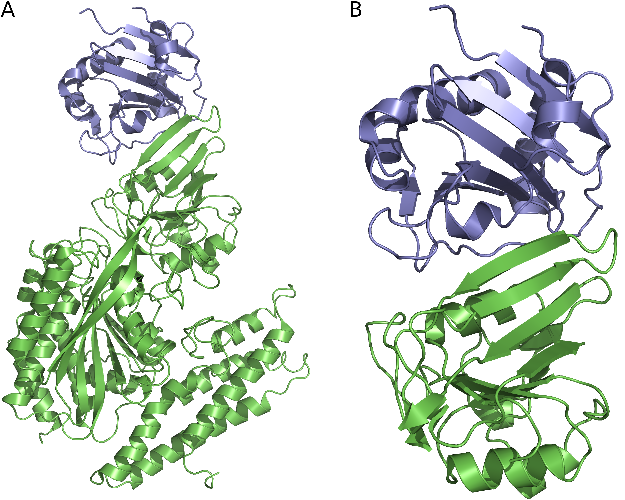
\includegraphics[width=6in]{figures/protein_comparison.pdf}}
\caption{\label{fig:protein_comparison}\title{Comparison of GP1/hTfR1 complex.} Figure A shows the full, de-glycosylated GP1/hTfR1 co-crystal structure. For figure B, we show the reduced structure for SMD. GP1 is blue and hTfR1 is green.}
\end{figure}

\clearpage
\begin{figure}[p]
\centerline{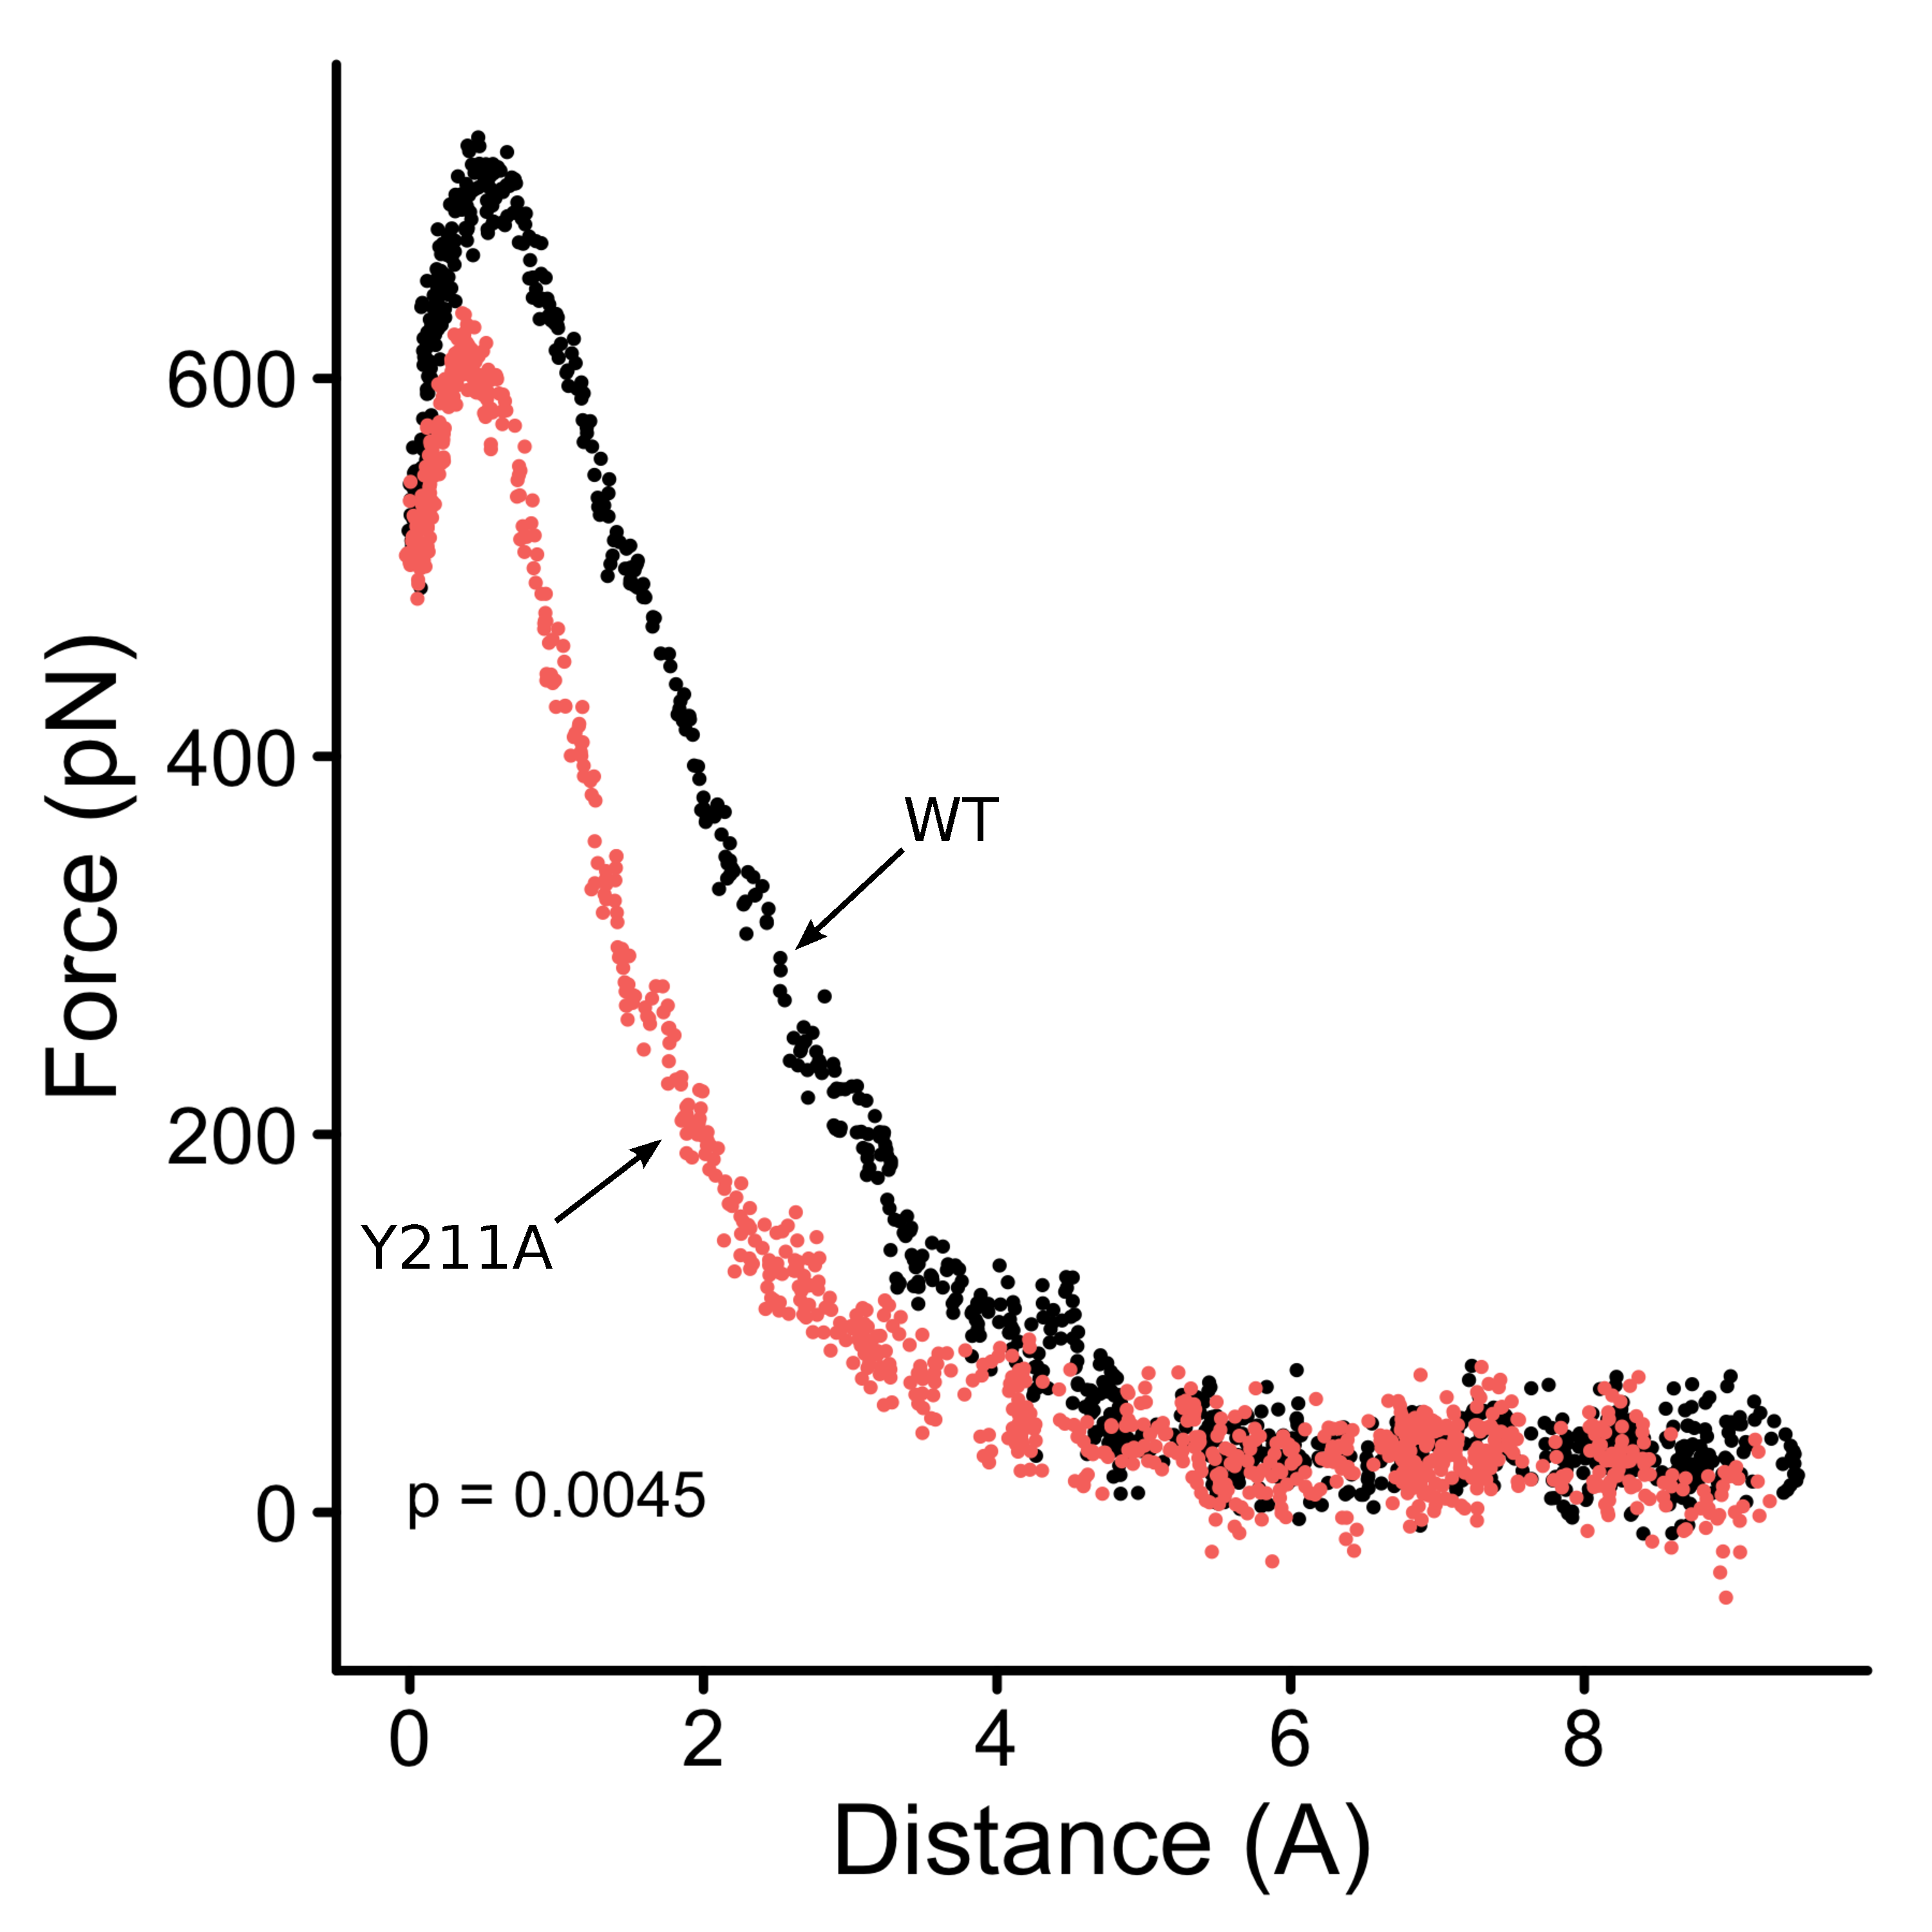
\includegraphics[width=6in]{figures/force_curve.pdf}}
\caption{\label{fig:force_curve}\title{Force versus distance curve of Y211A mutant and WT.} The average force curve for 50 replicates of the WT complex was black, and the average of 50 replicates of the Y211A mutant was red. Notice there is a very large difference in MAF and AUC between the two complexes.}
\end{figure}

\clearpage
\begin{figure}[p]
\centerline{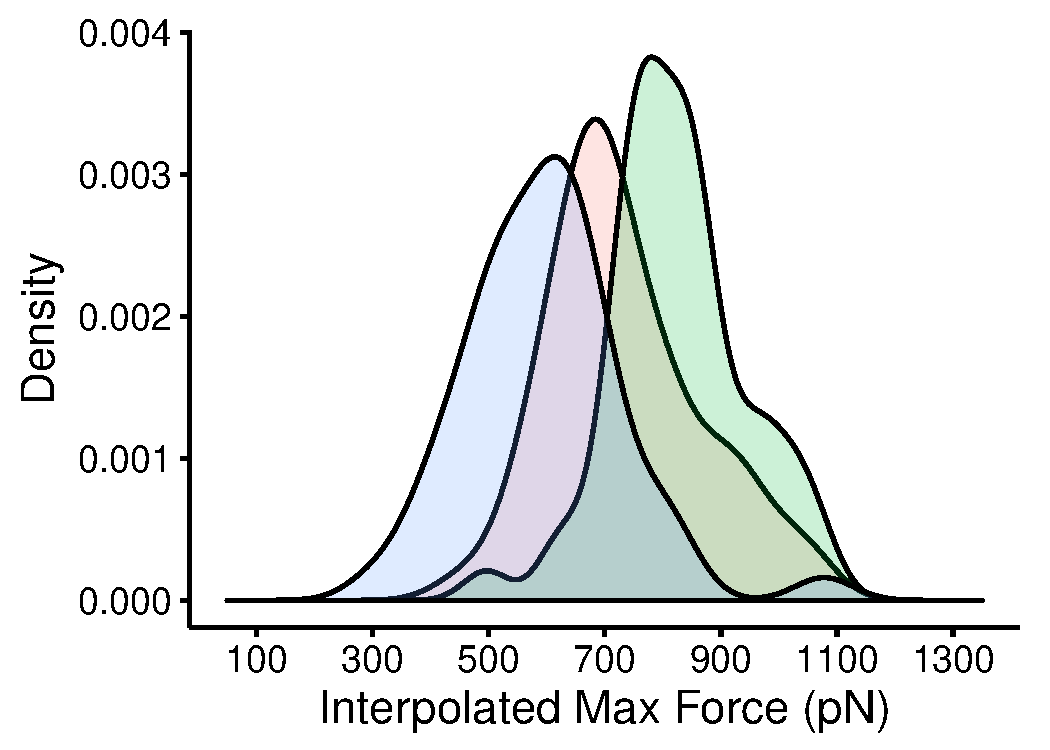
\includegraphics[width=6in]{figures/sensitivity_histogram.pdf}}
\caption{\label{fig:sensitivity}\title{Density plot of three different GP1/hTfR1 complexes.} The WT GP1-hTfR1 complex in the middle is flanked by the tighter binding mutant Y211D on the right and the weaker binding double mutant N348W/Y211A on the left. The large non-overlapping areas indicate a large and statistically significant difference in these three complexes with relatively minor differences.}
\end{figure}

\clearpage
\begin {table}[H]
\caption{\label{tab:summary_statistics}Summary statistics for each mutation tested. $\mu_\text{MAF}$ is the mean and $\sigma_\text{MAF}$ is the standard deviation of MAF over all simulations. $\mu_\text{AUC}$ is the mean and $\sigma_\text{AUC}$ is the standard deviation of AUC over all simulations.}
\begin{center}
  \resizebox{11cm}{!} {
    \begin{tabular}{l r r r r}
    \hline
      Mutation &      $\mu_\text{MAF}$ & $\sigma_\text{MAF}$ & $\mu_\text{AUC}$ & $\sigma_\text{AUC}$ \\ \hline
            WT &                 772.00 & 154.13               & 198794.7    & 66765.64 \\
         N348A &                 799.33 & 154.36               & 202247.3    & 65175.78 \\
         N348K &                 731.36 & 151.01               & 179087.5    & 55799.49 \\
         N348W &                 732.13 & 131.21               & 192043.2    & 66916.36 \\
        vR111A &                 754.39 & 103.25               & 185896.8    & 46408.74 \\
         Y211A &                 684.03 & 126.69               & 153517.7    & 40889.12 \\ 
         Y211D &                 875.44 & 116.46               & 234909.3    & 50494.11 \\ 
         Y211T &                 861.17 & 158.48               & 231078.7    & 97569.29 \\
   N348A/Y211A &                 762.96 & 144.81               & 173059.2    & 59898.10 \\
   N348W/Y211A &                 617.21 & 163.33               & 147705.6    & 48548.61 \\
  vR111A/Y211A &                 780.71 & 135.65               & 189919.1    & 48868.16 \\
    \hline
    \end{tabular}
  }
\end{center}
\end{table}

\clearpage
\begin {table}[H]
\caption{\label{tab:pairwise_differences}Pairwise differences (row variable minus column variable) in mean MAF. Bolded values are statistically significant at $p<0.05$. Values marked with * and ** are significant at $p<0.01$ and $p<0.001$, respectively.}
\begin{center}
  \resizebox{16cm}{!} {
    \begin{tabular}{l l l l l l l l l l l}
    \hline
                & WT                  & N348A              & N348W              & N348K              & Y211A             & Y211D              & Y211T              & vR111A             & N348A/Y211A        & N348W/Y211A        \\ \hline
    N348A       &  27.33              &                    &                    &                    &                   &                    &                    &                    &                    &                    \\
    N348W       & -39.87              & \textbf{-67.20}    &                    &                    &                   &                    &                    &                    &                    &                    \\
    N348K       & -40.64              & \textbf{-67.97}    & -0.77              &                    &                   &                    &                    &                    &                    &                    \\
    Y211A       & \textbf{-87.97*}    & \textbf{-115.30**} & -48.10             & -47.33             &                   &                    &                    &                    &                    &                    \\
    Y211D       & \textbf{103.44**}   & \textbf{76.12*}    & \textbf{143.31**}  & \textbf{144.08**}  & \textbf{191.42**} &                    &                    &                    &                    &                    \\
    Y211T       & \textbf{89.17*}     & \textbf{61.85}     & \textbf{129.04**}  & \textbf{129.81**}  & \textbf{177.15**} & -14.27             &                    &                    &                    &                    \\
   vR111A       & -17.76              & -44.94             & 22.26              & 23.03              & \textbf{70.36}    & \textbf{-121.05**} & \textbf{-106.78**} &                    &                    &                    \\
    N348A/Y211A & -9.04               & -36.37             & 30.83              & 31.60              & \textbf{78.93}    & \textbf{-112.48**} & \textbf{-98.21*}   & 8.57               &                    &                    \\
    N348W/Y211A & \textbf{-154.79**}  & \textbf{-182.12**} & \textbf{-114.92**} & \textbf{-114.15**} & \textbf{-66.2}    & \textbf{-258.23**} & \textbf{-243.96**} & \textbf{-137.18**} & \textbf{-145.75**} &                    \\
   vR111A/Y211A &  8.71               & -18.12             & 48.58              & 49.35              & \textbf{96.68*}   & \textbf{-94.74*}   & \textbf{-80.46*}   & 26.31              & 0.59               & \textbf{163.50**} \\
    \hline
    \end{tabular}
  }
\end{center}
\end{table}

\iffalse
\begin {table}[H]
\caption{Pairwise difference $p-$values for interpolated AUC. Bolded values are statistically significant at $p<0.05$.}
\begin{center}
  \resizebox{16cm}{!} {
    \begin{tabular}{l l l l l l l l l l l}
    \hline
                & WT               & N348A                   & N348W           & N348K                   & Y211A                   & Y211D                   & Y211T                   & vR111A          & N348A/Y211A & N348W/Y211A \\ \hline
    N348A       & 0.77             &                         &                 &                         &                         &                         &                         &                 &             &        \\
    N348W       & 0.67             & 0.42                    &                 &                         &                         &                         &                         &                 &             &        \\
    N348K       & 0.17             & 0.056                   & 0.38            &                         &                         &                         &                         &                 &             &        \\
    Y211A       & \textbf{0.00094} & \textbf{3.5x10$^{-05}$} & \textbf{0.0045} & 0.063                   &                         &                         &                         &                 &             &        \\
    Y211D       & \textbf{0.0072}  & \textbf{0.0051}         & \textbf{0.0016} & \textbf{4.6x10$^{-05}$} & \textbf{1.2x10$^{-09}$} &                         &                         &                 &             &        \\
    Y211T       & \textbf{0.016}   & \textbf{0.014}          & \textbf{0.0041} & \textbf{0.00016}        & \textbf{6.1x10$^{-09}$} & 0.77                    &                         &                 &             &        \\
   vR111A       & 0.38             & 0.18                    & 0.68            & 0.67                    & \textbf{0.016}          & \textbf{0.00032}        & \textbf{0.00094}        &                 &             &        \\
    N348A/Y211A & 0.061            & \textbf{0.013}          & 0.18            & 0.68                    & 0.17                    & \textbf{5.2x10$^{-06}$} & \textbf{2.1$^{-05}$}    & 0.38            &             &        \\
    N348W/Y211A & \textbf{0.00017} & \textbf{3.9x10$^{-06}$} & \textbf{0.0011} & \textbf{0.021}          & 0.68                    & \textbf{1.6x10$^{-10}$} & \textbf{6.3x10$^{-10}$} & \textbf{0.0047} & 0.063       &        \\
   vR111A/Y211A & 0.56             & 0.34                    & 0.86            & 0.47                    & \textbf{0.0072}         & \textbf{0.0010}         & \textbf{0.0025}         & 0.77            & 0.24        & \textbf{0.0019}  \\
    \hline
    \end{tabular}
  }
\end{center}
\end{table}
\fi

% \clearpage
% \begin {table}[H]\label{tab:
% \caption{Pairwise differences in interpolated MAF. Bolded values are statistically significant at $p<0.05$. $\Delta$ Max Force is the mean MAF for the first mutant listed in a row minus that of the second mutant listed.}
% \begin{center}
%   \resizebox{14cm}{!} {
%     \begin{tabular}{l r}
%     \hline
%     Mutant Pair                &  $\Delta$ Max Force \\ \hline
%     N348A-WT                   &               27.33 \\
%     N348W-WT                   &              -39.87 \\
%     N348K-WT                   &              -40.64 \\
%     \textbf{Y211A-WT}          &      \textbf{-87.97} \\
%     \textbf{Y211D-WT}          &      \textbf{103.44} \\
%     \textbf{Y211T-WT}          &       \textbf{89.17} \\
%     vR111A-WT                  &              -17.61 \\
%     N348A/Y211A-WT             &               -9.04 \\
%     \textbf{N348W/Y211A-WT}    &     \textbf{-154.79} \\
%     vR111A/Y211A-WT            &                8.71 \\
%     \textbf{N348W-N348A}       &      \textbf{-67.20} \\
%     \textbf{N348K-N348A}       &      \textbf{-67.97} \\
%     \textbf{Y211A-N348A}       &     \textbf{-115.30} \\
%     \textbf{Y211D-N348A}       &       \textbf{76.12} \\
%     \textbf{Y211T-N348A}       &       \textbf{61.85} \\
%     vR111A-N348A               &              -44.94 \\
%     N348A/Y211A-N348A          &              -36.37 \\
%     \textbf{N348W/Y211A-N348A} &     \textbf{-182.12} \\
%     vR111A/Y211A-N348A         &              -18.62 \\
%     N348K-N348W                &               -0.77 \\
%     Y211A-N348W                &              -48.10 \\
%     \textbf{Y211D-N348W}       &      \textbf{143.31} \\
%     \textbf{Y211T-N348W}       &      \textbf{129.04} \\
%     vR111A-N348W               &               22.26 \\
%     N348A/Y211A-N348W          &               30.83 \\
%     \textbf{N348W/Y211A-N348W} &     \textbf{-114.92} \\
%     vR111A/Y211A-N348W         &               48.58 \\
%     Y211A-N348K                &              -47.33 \\
%     
%     \hline
%     \end{tabular}
%     
%     \begin{tabular}{l r}
%     \hline
%     Mutant Pair                       &  $\Delta$ Max Force  \\ \hline
%     \textbf{Y211D-N348K}              &      \textbf{144.08} \\
%     \textbf{Y211T-N348K}              &      \textbf{129.81} \\
%     vR111A-N348K                      &               23.03  \\
%     N348A/Y211A-N348K                 &               31.60  \\
%     \textbf{N348W/Y211A-N348K}        &     \textbf{-114.15} \\
%     vR111A/Y211A-N348K                &               49.35  \\
%     \textbf{Y211D-Y211A}              &      \textbf{191.42} \\
%     \textbf{Y211T-Y211A}              &      \textbf{177.15} \\
%     \textbf{vR111A-Y211A}             &       \textbf{70.36} \\
%     \textbf{N348A/Y211A-Y211A}        &       \textbf{78.93} \\
%     \textbf{N348W/Y211A-Y211A}        &      \textbf{-66.82} \\
%     \textbf{vR111A/Y211A-Y211A}       &       \textbf{96.68} \\
%     Y211T-Y211D                       &              -14.27  \\
%     \textbf{vR111A-Y211D}             &     \textbf{-121.05} \\
%     \textbf{N348A/Y211A-Y211D}        &     \textbf{-112.48} \\
%     \textbf{N348W/Y211A-Y211D}        &     \textbf{-258.23} \\
%     \textbf{vR111A/Y211A-Y211D}       &      \textbf{-94.74} \\
%     \textbf{vR111A-Y211T}             &     \textbf{-106.78} \\
%     \textbf{N348A/Y211A-Y211T}        &      \textbf{-98.21} \\
%     \textbf{N348W/Y211A-Y211T}        &     \textbf{-243.96} \\
%     \textbf{vR111A/Y211A-Y211T}       &      \textbf{-80.46} \\
%     N348A/Y211A-vR111A                &                8.57  \\
%     \textbf{N348W/Y211A-vR111A}       &     \textbf{-137.18} \\
%     vR111A/Y211A-R111A                &               26.31  \\
%     \textbf{N348W/Y211A-N348A/Y211A}  &     \textbf{-145.75} \\
%     vR111A/Y211A-N348A/Y211A          &               17.75  \\
%     \textbf{vR111A/Y211A-N348W/Y211A} &      \textbf{163.50} \\ 
%                                       &          \\
%     \hline
%     \end{tabular}
%   }
% \end{center}
% \end{table}

\clearpage
\begin {table}[H]
\caption{\label{tab:MAF_p}Pairwise difference $p-$values for MAF. Bolded values are statistically significant at $p<0.05$.}
\begin{center}
  \resizebox{16cm}{!} {
    \begin{tabular}{l l l l l l l l l l l}
    \hline
                & WT                      & N348A                   & N348W                   & N348K                   & Y211A                   & Y211D                     & Y211T                   & vR111A                  & N348A/Y211A             & N348W/Y211A \\ \hline
    N348A       & 0.35                    &                         &                         &                         &                         &                           &                         &                         &                         &        \\
    N348W       & 0.22                    & \textbf{0.012}          &                         &                         &                         &                           &                         &                         &                         &        \\
    N348K       & 0.22                    & \textbf{0.012}          & 0.98                    &                         &                         &                           &                         &                         &                         &        \\
    Y211A       & \textbf{0.0045}         & \textbf{1.6x10$^{-05}$} & 0.14                    & 0.15                    &                         &                           &                         &                         &                         &        \\
    Y211D       & \textbf{0.00083}        & \textbf{0.0045}         & \textbf{3.9x10$^{-06}$} & \textbf{3.9x10$^{-06}$} & \textbf{5.7x10$^{-10}$} &                           &                         &                         &                         &        \\
    Y211T       & \textbf{0.0042}         & \textbf{0.022}          & \textbf{3.0x10$^{-05}$} & \textbf{3.0x10$^{-05}$} & \textbf{1.0x10$^{-08}$} & 0.67                      &                         &                         &                         &        \\
   vR111A       & 0.59                    & 0.11                    & 0.51                    & 0.51                    & \textbf{0.024}          & \textbf{8.9x10$^{-05}$}   & \textbf{0.00056}        &                         &                         &        \\
    N348A/Y211A & 0.78                    & 0.20                    & 0.35                    & 0.35                    & \textbf{0.011}          & \textbf{0.00026}          & \textbf{0.0016}         & 0.78                    &                         &        \\
    N348W/Y211A & \textbf{6.2x10$^{-07}$} & \textbf{9.3x10$^{-12}$} & \textbf{0.00021}        & \textbf{0.00026}        & \textbf{0.032}          & \textbf{$<$ 2x10$^{-16}$} & \textbf{2.4x10$^{-15}$} & \textbf{9.1x10$^{-06}$} & \textbf{2.8x10$^{-06}$} &        \\
   vR111A/Y211A & 0.78                    & 0.52                    & 0.14                    & 0.14                    & \textbf{0.0019}         & \textbf{0.0024}           & \textbf{0.010}          & 0.44                    & 0.59                    & \textbf{1.6x10$^{-07}$}  \\
    \hline
    \end{tabular}
  }
\end{center}
\end{table}

\begin {table}[H]
\caption{\label{tab:AUC_p}Pairwise difference $p-$values for interpolated AUC. Bolded values are statistically significant at $p<0.05$.}
\begin{center}
  \resizebox{16cm}{!} {
    \begin{tabular}{l l l l l l l l l l l}
    \hline
                & WT               & N348A                   & N348W           & N348K                   & Y211A                   & Y211D                   & Y211T                   & vR111A          & N348A/Y211A & N348W/Y211A \\ \hline
    N348A       & 0.77             &                         &                 &                         &                         &                         &                         &                 &             &        \\
    N348W       & 0.67             & 0.42                    &                 &                         &                         &                         &                         &                 &             &        \\
    N348K       & 0.17             & 0.056                   & 0.38            &                         &                         &                         &                         &                 &             &        \\
    Y211A       & \textbf{0.00094} & \textbf{3.5x10$^{-05}$} & \textbf{0.0045} & 0.063                   &                         &                         &                         &                 &             &        \\
    Y211D       & \textbf{0.0072}  & \textbf{0.0051}         & \textbf{0.0016} & \textbf{4.6x10$^{-05}$} & \textbf{1.2x10$^{-09}$} &                         &                         &                 &             &        \\
    Y211T       & \textbf{0.016}   & \textbf{0.014}          & \textbf{0.0041} & \textbf{0.00016}        & \textbf{6.1x10$^{-09}$} & 0.77                    &                         &                 &             &        \\
   vR111A       & 0.38             & 0.18                    & 0.68            & 0.67                    & \textbf{0.016}          & \textbf{0.00032}        & \textbf{0.00094}        &                 &             &        \\
    N348A/Y211A & 0.061            & \textbf{0.013}          & 0.18            & 0.68                    & 0.17                    & \textbf{5.2x10$^{-06}$} & \textbf{2.1$^{-05}$}    & 0.38            &             &        \\
    N348W/Y211A & \textbf{0.00017} & \textbf{3.9x10$^{-06}$} & \textbf{0.0011} & \textbf{0.021}          & 0.68                    & \textbf{1.6x10$^{-10}$} & \textbf{6.3x10$^{-10}$} & \textbf{0.0047} & 0.063       &        \\
   vR111A/Y211A & 0.56             & 0.34                    & 0.86            & 0.47                    & \textbf{0.0072}         & \textbf{0.0010}         & \textbf{0.0025}         & 0.77            & 0.24        & \textbf{0.0019}  \\
    \hline
    \end{tabular}
  }
\end{center}
\end{table}

\end{document}
